\subsection{Some theory on SMO convergence}
Let $\alpha$ be some feasible variable for Problem (\ref{eq:dual_problem}). Defining
\begin{align*}
\mathcal{L}(\alpha,\delta,\mu,\beta) &:= \frac{1}{2} \alpha^T Q \alpha - 1^T \alpha - \delta^T\alpha + \mu^T(\alpha - C) - \beta \alpha^T y \\
F_i(\alpha) &:= y_i (\partial_i d)(\alpha) = \sum_{i = 1}^l \alpha_j y_j k(x_i,x_j) - y_i \quad \text{for} \quad i = 1,\ldots,l,
\end{align*}
by careful manipulations we find that the KKT optimality conditions
\begin{equation*}
\left.
\begin{aligned}
\nabla_{\alpha} \mathcal{L}(\alpha^*,\delta^*,\mu^*,\beta^*) &= 0\\
\delta_i^* &\geq 0\\
\delta_i^* \alpha_i^* &= 0\\
\mu_i^* &\geq 0\\
\mu_i^* (\alpha_i^*-C) &= 0\\
\alpha_i^* &\text{ feasible}
\end{aligned}
\right\} \text{for all } i \in \{1,\ldots,l\}
\end{equation*}
for a solution of Problem (\ref{eq:dual_problem}) (which are sufficient, since Q is spsd), are equivalent to the -- much simpler looking -- pairwise condition
\begin{equation*}\label{equiv_KKT}
b_{up}(\alpha) := \min_{i \in I_{up}(\alpha)} F_i(\alpha) \geq \max_{j \in I_{low}(\alpha)} F_j(\alpha) =: b_{low}(\alpha),
\end{equation*}
where $I_{up}(\alpha)$ and $I_{low}(\alpha)$ are subsets of the index set $\{1,\ldots,l\}$ defined by
\begin{align*}
I_{up}(\alpha) &:= \{ i  \mid  \alpha_i < C \text{ and } y_i = 1 \text{ or } \alpha_i > 0 \text{ and } y_i = -1 \} \\
I_{low}(\alpha) &:= \{ j \mid \alpha_j < C \text{ and } y_j = -1 \text{ or } \alpha_j > 0 \text{ and } y_j = 1 \}.
\end{align*} 
Any pair $(i,j) \in I_{up}(\alpha) \times I_{low}(\alpha)$ with $F_i(\alpha) < F_j(\alpha)$ is thus called a \textit{violating pair} and an objective equivalent to solving Problem (\ref{eq:dual_problem}) is to change $\alpha$ so as to remove all such violating pairs. Since a priori we do not know if the solution $\alpha^*$ fulfils (\ref{equiv_KKT}) strictly or not, we define, for some small tolerance $\tau > 0$, a $\tau$-violating pair as some $(i,j) \in I_{up}(\alpha) \times I_{low}(\alpha)$ which satisfies $F_i(\alpha) < F_j(\alpha) - \tau$ and require that all $\tau$-violating pairs be removed, or equivalently, 
\begin{equation*}\label{tau_KKT}
b_{up}(\alpha) \geq b_{low}(\alpha) - \tau.
\end{equation*}
It holds (see \cite{Keerthi2002} for a proof) that any algorithm of the following form terminates after finitely many steps:
\begin{algorithm}[General SMO type algorithm]\label{GSMO} Let $\tau > 0$. Initialize $k = 0 $ and $\alpha^0 = 0$ and generate iterates $\alpha^k$, $k \in \mathbb{N},$ as follows: 
\begin{enumerate}
\item If $\alpha^k$ satisfies (\ref{tau_KKT}), stop. Else choose a $\tau$-violating pair $(i,j) \in I_{up}(\alpha^k) \times I_{low}(\alpha^k)$.
\item Minimize $d$ varying only $\alpha^k_i$ and $\alpha^k_j$, leaving $\alpha^k_n$ fixed for $n \notin \{i,j\}$ and respecting the constraints of Problem (\ref{eq:dual_problem}) to obtain $\alpha^{\text{new}}$.
\item Set $k := k+1$, $\alpha^k := \alpha^{\text{new}}$ and go to Step 1.
\end{enumerate}
\end{algorithm} 
Platt's original Sequential Minimal Optimization (SMO) algorithm (actually, we are referring to "Modification 1" by \cite{KeerthiShevade}), although ground-breaking, has two weaknesses. Firstly, its pseudocode description is quite complex, making it hard to judge whether or not one has implemented it as intended by its originators. Secondly, by trying to avoid computational effort in the \textit{while} steps, it actually runs much longer than all other algorithms we have implemented or tested.\\\\
In short, Platt's SMO tries first to ensure that
\[
b_{up,I_0}(\alpha) := \max_{i \in I_0(\alpha)} F_i(\alpha) \geq \min_{j \in I_0} F_j(\alpha) =: b_{low,I_0}(\alpha),
\]
where $I_0(\alpha) := \{ i  \mid  0 < \alpha_i < C \}$ is the index set of ``interior'' $\alpha_i$s. A cache of only the $F_i$ for $i \in I_0$ is kept until this is achieved. Then all $i \in \{0,\ldots l\}$ are examined, and the cache of correctly stored $F_i$s (along with the indices $\widetilde{i_{up}}$ and $\widetilde{i_{low}}$ indicating where the so far most extreme $F_i$ occur) is extended as long as an $\alpha_j$ is found such that $(j,\widetilde{i_{low}})$ or $(\widetilde{i_{up}},j)$ is violating, depending on whether $j \in I_{up}$ or $j \in I_{low}$.\\\\
Therefore, the algorithm does not resolve a \textit{maximally} violating pair, by which we mean some 
\[
(i_{up},i_{low}) \in \argmin_{i \in I_{up}(\alpha)}F_i(\alpha) \times \argmax_{j \in I_{low}(\alpha)}F_j(\alpha).
\] To look up such a pair is the strategy of the ``Working Set Selection 1'' (WSS1) approach in \cite{FanChenLin} and a rewarding investment, see benchmarking section. \\\\
Parametrize the 1D Problem in Step 2 of Algorithm \ref{GSMO} as
\[
\alpha_i(t^*) = \alpha^k_i + y_i t*, \quad \alpha_j(t^*) = \alpha^k_j - y_j t*, \quad \alpha_n(t^*) = \alpha^k_n \text{ for } k \notin \{i,j\}
\]
for some optimal feasible $t^* \in \R$ and set $\Phi(t) = d(\alpha(t))$ as the 1D objective function. Then actually
\begin{equation*}
F_i(\alpha) - F_j(\alpha) = \Phi'(0),
\end{equation*}
so WSS1 corresponds to a steepest descent approach aiming for a substantial decrease in $d$. Since this uses only first order information, a second ``Working Set Selection 2'' (WSS2) strategy is proposed in \cite{FanChenLin}, which (at relatively low extra cost) employs second order information to choose a violating pair almost optimally: $i \in \argmin_{i \in I_{up}(\alpha)}F_i(\alpha)$ and $j \in I_{low}$ such that the decrease in $d$ produced by removing the violating pair is maximal.

\subsection{Implementational issues}
One particular source of trouble was that WSS1 and WSS2 sometimes got stuck on a single violating pair, which is extremely puzzling because -- in theory -- a violating pair $(i,j)$ of indices can no longer be violating after an SMO step has been taken. It turned out that the precise definitions of $I_{up}$ and $I_{low}$ had to be softened so that numerical errors do not stop the algorithm from recognizing that $(\alpha^{new}_i,\alpha^{new}_j$ has hit the boundary of $[0,C]^2$. This is crucial for steps where the box constraints are active for $(\alpha^{new}_i,\alpha^{new}_j)$. For further details, please see the commented code we provided. 

\subsection{Benchmarking different SMOs}

We implemented Platt's SMO, WSS1 in two variations and WSS2. The first variation of WSS1 caches all computations of Gramian matrix rows in order to avoid expensive double computations. The other variant of WSS1 is forgetful. Taking the scikit-learn SVC algorithm as a 5th (tough) competitor, we tested the algorithms at hand for the first classifier of ECOC for a range of numbers of MNIST training points. \\\\
As can be seen, the speediest algorithms are, in decreasing order: scikit-learn, WSS1 with caching, WSS2 with caching, WSS1 without caching, Platt's SMO. Somewhat surprisingly, WSS2 with caching is not the fastest method, although in theory it should be superior to WSS1 with caching. Apparently, the extra computational cost outweighs the theoretical gain. We suppose that the strange kink in the WSS1 with caching graph (Figure \ref{bench_ssp}) is due to multicore features of Python kicking in at 1800 training points. The benchmarks were carried out on a Windows 7 x64 machine with an Intel i5 quad core processor at 4 GHz and 16 GB of RAM.\\\\
The polynomial order of all algorithms is 2, judging from the loglog plot in Figure \ref{bench_gauss_loglog} and a linear least squares fit of the loglog data for WSS1 with caching. The latter also yielded that our WSS1 with caching takes about 5.8 times as long as scikit-learn.

\begin{figure}[h!]
	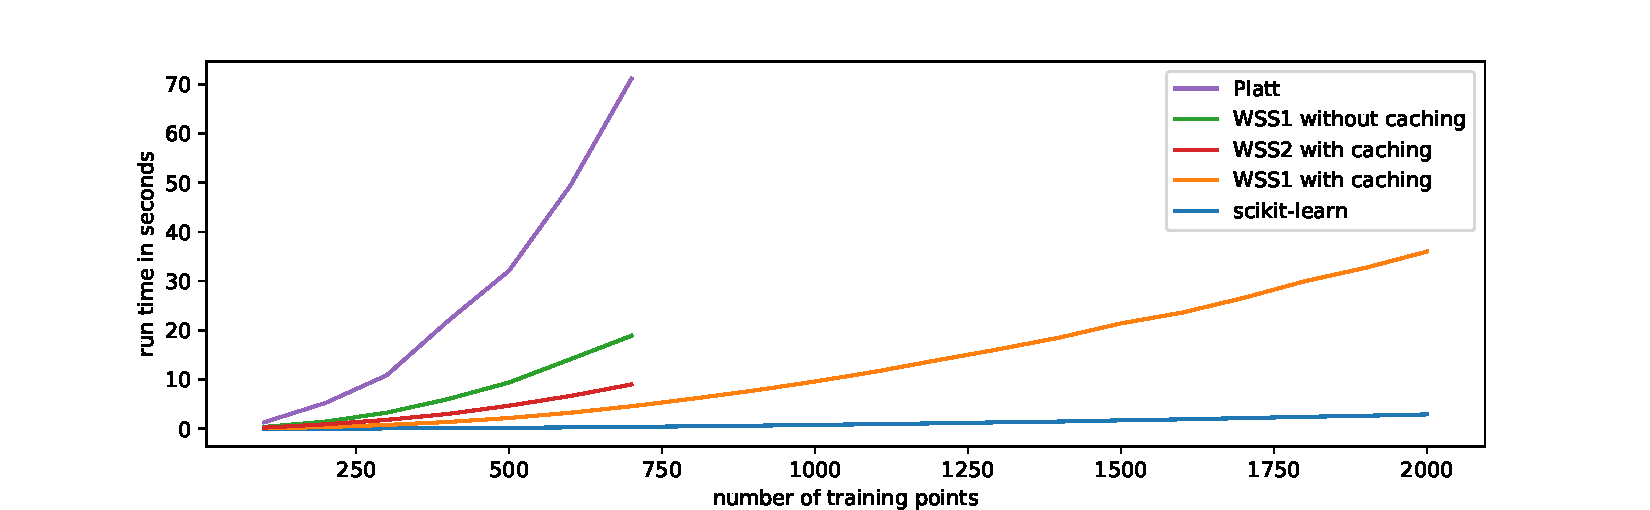
\includegraphics[width=1\textwidth, center]{benchplot_gauss.pdf}
	\caption{Run times for different SMO algorithms, Gaussian kernel}
	\label{bench_gauss}
\end{figure}

\begin{figure}[h!]
	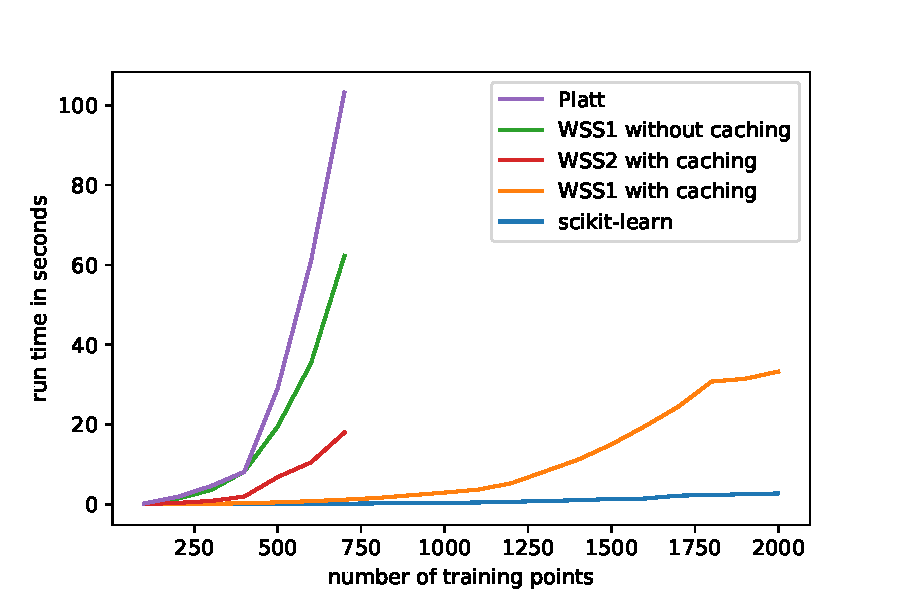
\includegraphics[width=1\textwidth, center]{benchplot_ssp.pdf}
	\caption{Run times for different SMO algorithms, standard scalar product}
	\label{bench_ssp}
\end{figure}

\begin{figure}[h!]
	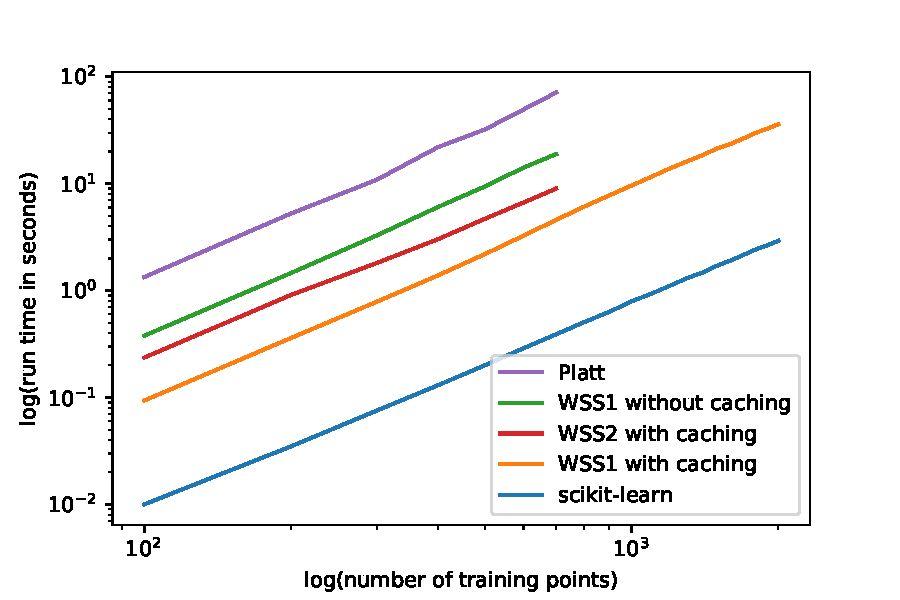
\includegraphics[width=1\textwidth, center]{benchplot_gauss_loglog.pdf}
	\caption{loglog plot of run times, Gaussian kernel}
	\label{bench_gauss_loglog}
\end{figure}





\newpage